\documentclass[11pt,a4paper,oneside]{report}
% SEVEN embedded systems technical report - editable LaTeX source.
% Compile with: pdflatex main.tex (twice) or upload the entire folder to Overleaf.
% Do not treat simulated outputs as measured hardware results.
\usepackage[T1]{fontenc}
\usepackage[utf8]{inputenc}
\usepackage{lmodern}
\usepackage[english]{babel}
\usepackage{geometry}
\geometry{left=26mm,right=24mm,top=26mm,bottom=27mm}
\usepackage{microtype}
\usepackage{amsmath,amssymb}
\usepackage{booktabs,tabularx,longtable,array,multirow}
\usepackage[table]{xcolor}
\usepackage{graphicx}
\usepackage{subcaption}
\usepackage{float}
\usepackage{placeins}
\usepackage{tikz}
\usetikzlibrary{arrows.meta,positioning,shapes.geometric,calc}
\usepackage{enumitem}
\usepackage{fancyhdr}
\usepackage{hyperref}
\usepackage{listings}
\usepackage[most]{tcolorbox}
\usepackage{caption}
\usepackage{titlesec}
\usepackage{lastpage}
\usepackage{url}
\definecolor{navy}{HTML}{132A46}
\definecolor{teal}{HTML}{097D86}
\definecolor{muted}{HTML}{54657A}
\definecolor{pale}{HTML}{E9F3F4}
\definecolor{amber}{HTML}{A36213}
\definecolor{papergray}{HTML}{F4F7FA}
\definecolor{darktext}{HTML}{263242}
\newcommand{\TeamMembers}{Assia Snissi, Khadija Lekbiri, Manal Zaidi, Rhita Rhallami}
\hypersetup{colorlinks=true,linkcolor=navy,urlcolor=teal,citecolor=teal,pdftitle={SEVEN Industrial Color-Sorting MVP - Embedded Systems Report},pdfauthor={\TeamMembers}}
\setlength{\parindent}{0pt}
\setlength{\parskip}{5.5pt}
\setcounter{secnumdepth}{3}
\setcounter{tocdepth}{2}
\setlist[itemize]{leftmargin=*,topsep=2pt,itemsep=3pt}
\setlist[enumerate]{leftmargin=*,topsep=2pt,itemsep=3pt}
\renewcommand{\arraystretch}{1.18}
\titleformat{\chapter}[display]{\normalfont\bfseries\color{navy}}{\fontsize{11}{12}\selectfont CHAPTER \thechapter}{6pt}{\Huge}
\titlespacing*{\chapter}{0pt}{-18pt}{18pt}
\titleformat{\section}{\Large\bfseries\color{navy}}{\thesection}{.6em}{}
\titleformat{\subsection}{\large\bfseries\color{teal}}{\thesubsection}{.6em}{}
\captionsetup{font=small,labelfont={bf,color=navy}}
\pagestyle{fancy}
\fancyhf{}
\fancyhead[L]{\small\textcolor{muted}{SEVEN \textbar\ Embedded Systems}}
\fancyhead[R]{\small\textcolor{muted}{UM6P College of Computing}}
\fancyfoot[L]{\footnotesize\textcolor{muted}{Technical report v2.0 \textbar\ November 2026}}
\fancyfoot[R]{\footnotesize\textcolor{muted}{\thepage\ / \pageref{LastPage}}}
\renewcommand{\headrulewidth}{0.35pt}
\setlength{\headheight}{15pt}
\fancypagestyle{plain}{\fancyhf{}\fancyfoot[R]{\footnotesize\textcolor{muted}{\thepage\ / \pageref{LastPage}}}\renewcommand{\headrulewidth}{0pt}}
\lstdefinestyle{project}{basicstyle=\ttfamily\footnotesize,backgroundcolor=\color{papergray},frame=single,rulecolor=\color{teal!20},breaklines=true,columns=fullflexible,showstringspaces=false,commentstyle=\color{muted},keywordstyle=\color{teal},tabsize=2,xleftmargin=4pt,xrightmargin=4pt}
\lstset{style=project}
\newtcolorbox{note}[1][]{colback=pale,colframe=teal!65,boxrule=.65pt,arc=2mm,fonttitle=\bfseries,title={Engineering note},#1}
\newcommand{\Repo}{\url{https://github.com/elevenMiles/Robotic_Arm_Seven}}

\newcommand{\ModuleName}{Embedded Systems}

\newcommand{\Professor}{Professor Sadek}
\begin{document}
\pagenumbering{roman}
\begin{titlepage}
\pagecolor{navy}
\color{white}
\sffamily\raggedright
\setlength{\parskip}{0pt}
\vspace*{8mm}
{\large\bfseries Mohammed VI Polytechnic University\par}
\vspace{2mm}
{\normalsize College of Computing \enspace\textbar\enspace Embedded Systems\par}
\vfill
{\color{teal!35!white}\rule{20mm}{2pt}\par}
\vspace{7mm}
{\fontsize{52}{56}\selectfont\bfseries SEVEN\par}
\vspace{3mm}
{\fontsize{27}{32}\selectfont Vision-Guided Color Sorting\par}
\vspace{6mm}
{\large\color{teal!25!white} Industrial Sorting MVP \enspace\textbar\enspace Technical Project Report\par}
\vfill
{\small\bfseries\color{teal!35!white} PROJECT TEAM\par}
\vspace{3mm}
{\large \TeamMembers\par}
\vspace{9mm}
{\color{white!45!navy}\rule{\linewidth}{.5pt}\par}
\vspace{3mm}
{\small \Professor\hfill Report 2.0 \enspace\textbar\enspace 19 November 2026\par}
\vspace*{6mm}
\end{titlepage}
\nopagecolor
\color{darktext}
\chapter*{Document control and evidence status}
\addcontentsline{toc}{chapter}{Document control and evidence status}
\begin{tabularx}{\textwidth}{@{}p{.34\textwidth}X@{}}\toprule
Project framing & Working minimum viable prototype (MVP) demonstrating a vision-guided industrial color-sorting workflow on an educational robotic arm.\\
Primary implemented pipeline & Camera classification, human-approved serial route check, Arduino pick-and-place through one configured drop-off point per color.\\
Reproducible engineering evidence & Nine-pose FK/IK consistency, MATLAB commanded trajectories, Simulink illustrative servo tracking, PyBullet generic replay, Raspberry Pi and Arduino state diagrams.\\
Capacity-management specification & Three color bins, each with nominal capacity three; independent software counters, unchanged color-specific drop coordinates, operator reconciliation, and a FULL guard.\\
Capacity controller & Each color uses one firmware destination for all three counts. Eleven host-side tests passed with simulated inputs.\\\bottomrule
\end{tabularx}
\begin{note}[title={Scope of the results}]
Route times and tool paths come from commanded joint angles. The route clock starts when the controller accepts the run command and ends at HOME.
\end{note}
\chapter*{Abstract}
\addcontentsline{toc}{chapter}{Abstract}
SEVEN sorts a red, green or blue object from a fixed pickup point into its assigned bin. A Raspberry Pi classifies one camera frame and requests operator approval. An Arduino then drives three positioning servos and a gripper through eight waypoints. The engineering question is whether reaching each programmed waypoint is sufficient for a reliable pickup. All nine target poses pass the kinematic checks, yet the modeled tool moves sideways by 2.73 cm during a descent whose endpoints have identical horizontal coordinates. This makes clearance along the entire pickup path a design constraint. The modeled red, green and blue routes take 45.7, 43.1 and 49.5 s, respectively. Synthetic image tests exercise the color decision, and eleven host tests exercise capacity and recovery. 

\textbf{Keywords:} industrial sorting MVP; embedded systems; robotic manipulation; bin capacity; finite-state machines; HSV segmentation; Arduino; Raspberry Pi; MATLAB; Simulink; PyBullet.
\tableofcontents
\listoffigures
\listoftables
\clearpage
\pagenumbering{arabic}

\chapter{Introduction}
\section{Context and motivation}
Industrial sorting systems combine perception, decision-making and mechanical handling to route products according to observable properties. This project demonstrates those core functions as a small-scale, working MVP rather than a production-ready industrial machine. Even a three-degree-of-freedom (3-DOF) manipulator requires an explicit coordinate model, reliable communications and safe sequencing to transfer an object from a pickup point to a selected destination. This project uses color as the classification criterion and an inexpensive hobby-servo arm as the actuator platform.

The desired long-term application is automatic segregation of products on a larger line, but the prototype does not yet contain a conveyor, continuous acquisition or industrial sensors. The purpose is to validate the smallest working perception-to-actuation loop first.

The starting hardware is the open-source \emph{SEVEN} arm, published by T. Selçuk Yüksel, a 3D-printed Arduino-based mechanism with three positioning degrees of freedom and a gripper \cite{seven}. Our team built upon that platform with a Raspberry Pi computer-vision stage and custom firmware for fixed pickup and color-dependent drop-off routes. The custom firmware described here is \emph{not} the upstream repository's original command protocol.

\section{Problem statement and objectives}
\textbf{Problem:} identify the color of an object in a defined camera region and command a robotic arm to relocate it to the correct color bin while making the computational model, control logic and software constraints inspectable.

The engineering objectives are to: (i) assemble and operate the arm, (ii) classify red/green/blue and reject insufficient color coverage, (iii) communicate route commands through a supervised serial protocol, (iv) model the arm and produce reachable joint targets, (v) document control flow as finite state machines, (vi) explore per-bin capacity management at three objects per color using unchanged drop locations, and (vii) verify agreement between the exported trajectories and their 3D replay.

\section{Scope and contributions}
The present MVP uses a \textbf{single camera frame, fixed ROI, fixed pick location and one fixed drop location per color}. It is a human-confirmed sorting demonstration, not continuous visual tracking or autonomous object localization. The contributions described in this report are the Pi-to-Arduino interface, the eight-waypoint controller, reproducible MATLAB route computations, Simulink tracking illustrations, formal state diagrams and a PyBullet command replay.

\section{Structure of the report}
The report proceeds from requirements and hardware through camera processing, Arduino control, capacity-management design, kinematic modeling and finite-state machines. Later chapters document Simulink/PyBullet results, validation and limitations. Appendix A lists the project files and the commands used to reproduce the software checks.

\chapter{Requirements and System Architecture}
\section{Functional requirements}
\begin{table}[htbp]\centering\small
\caption{System-level functional requirements derived from the implementation and stated objective.}
\begin{tabularx}{\textwidth}{@{}p{.12\textwidth}X p{.22\textwidth}@{}}\toprule
ID & Requirement & Implemented component\\\midrule
FR-01 & Acquire a camera frame and evaluate a fixed image region. & Raspberry Pi/Picamera2\\
FR-02 & Classify RED/GREEN/BLUE and reject weak coverage as UNKNOWN. & OpenCV HSV masks\\
FR-03 & Request a non-moving route validity check before moving. & Serial \texttt{CHECK}\\
FR-04 & Require user confirmation before executing a recognized route. & Pi command script\\
FR-05 & Move through eight predefined pickup/transfer/drop waypoints. & Arduino firmware\\
FR-06 & Open and close the gripper at appropriate route phases. & Arduino gripper servo\\
FR-07 & Reproduce the commanded motion numerically for analysis. & MATLAB/Simulink\\
FR-08 & Visualize the color-specific sorting route in 3D. & PyBullet\\
FR-09 & Prevent more than three counted placements in a color bin. & Capacity extension\\
FR-10 & Reuse the color bin's existing fixed drop point for all three objects. & Fixed-drop host controller\\\bottomrule
\end{tabularx}\end{table}
\section{Non-functional requirements and constraints}
\begin{itemize}
\item \textbf{Reproducibility:} each route has a stored coordinate table, deterministic command schedule and CSV export.
\item \textbf{Observability:} text responses, saved ROI imagery, plotted commands and numerical checks make intermediate stages inspectable.
\item \textbf{Safety:} route reachability and command bounds are checked, but neither guarantees physical clearance; a human must supervise the arm.
\item \textbf{Low cost and accessibility:} a printed arm, hobby servos and readily available educational software are used.
\item \textbf{Reliability limits:} joint encoders, force sensors and collision feedback are not present in the reported setup.
\end{itemize}
\section{End-to-end architecture}
\begin{figure}[htbp]\centering
\resizebox{\textwidth}{!}{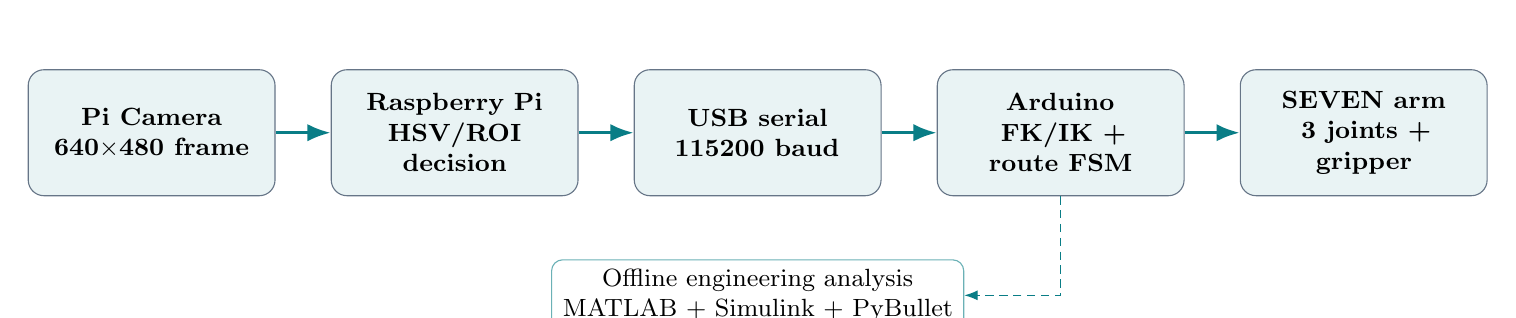
\begin{tikzpicture}[>=Latex,node distance=7mm,
  st/.style={draw=navy!65,rounded corners=2mm,fill=pale,minimum height=16mm,text width=29mm,align=center,font=\small\bfseries},
  ar/.style={-Latex,very thick,draw=teal}]
\node[st] (cam) {Pi Camera\\640$\times$480 frame};
\node[st,right=of cam] (cv) {Raspberry Pi\\HSV/ROI decision};
\node[st,right=of cv] (serial) {USB serial\\115200 baud};
\node[st,right=of serial] (ard) {Arduino\\FK/IK + route FSM};
\node[st,right=of ard] (servo) {SEVEN arm\\3 joints + gripper};
\draw[ar] (cam) -- (cv);\draw[ar] (cv) -- (serial);\draw[ar] (serial) -- (ard);\draw[ar] (ard) -- (servo);
\node[below=8mm of serial,draw=teal!60,rounded corners,fill=white,text width=50mm,align=center,font=\small] (model) {Offline engineering analysis\\MATLAB + Simulink + PyBullet};
\draw[densely dashed,teal,-Latex] (ard.south) |- (model.east);
\end{tikzpicture}}
\caption{Implemented control pipeline and separate offline modeling toolchain. The offline simulations do not control the live robot.}\label{fig:architecture}
\end{figure}
\section{Hardware/software separation}
The Raspberry Pi owns image acquisition and the decision to issue commands. The optional capacity layer is a host-side gate that allows or blocks a standard route; it must not be confused with the original single-shot camera script, which has no occupancy counter. The Arduino owns servo pulse generation, kinematic computations and nonblocking incremental motion. MATLAB and Simulink inspect the same nominal geometry and command sequence offline, while PyBullet provides a generic visualization. The model never claims to receive real encoder positions from the arm.

\chapter{Hardware and Integration}
\section{Robot and electronics}
The arm follows the SEVEN printed architecture \cite{seven}; three servos position the end effector (base, shoulder, elbow) and a fourth actuates the gripper. The team's previously reported arrangement uses a separate four-AA battery holder for the servo rail and a 5 V/3 A supply for the Raspberry Pi. Figure~\ref{fig:physical-setup} shows the assembled prototype on the test bench.

\begin{figure}[htbp]\centering
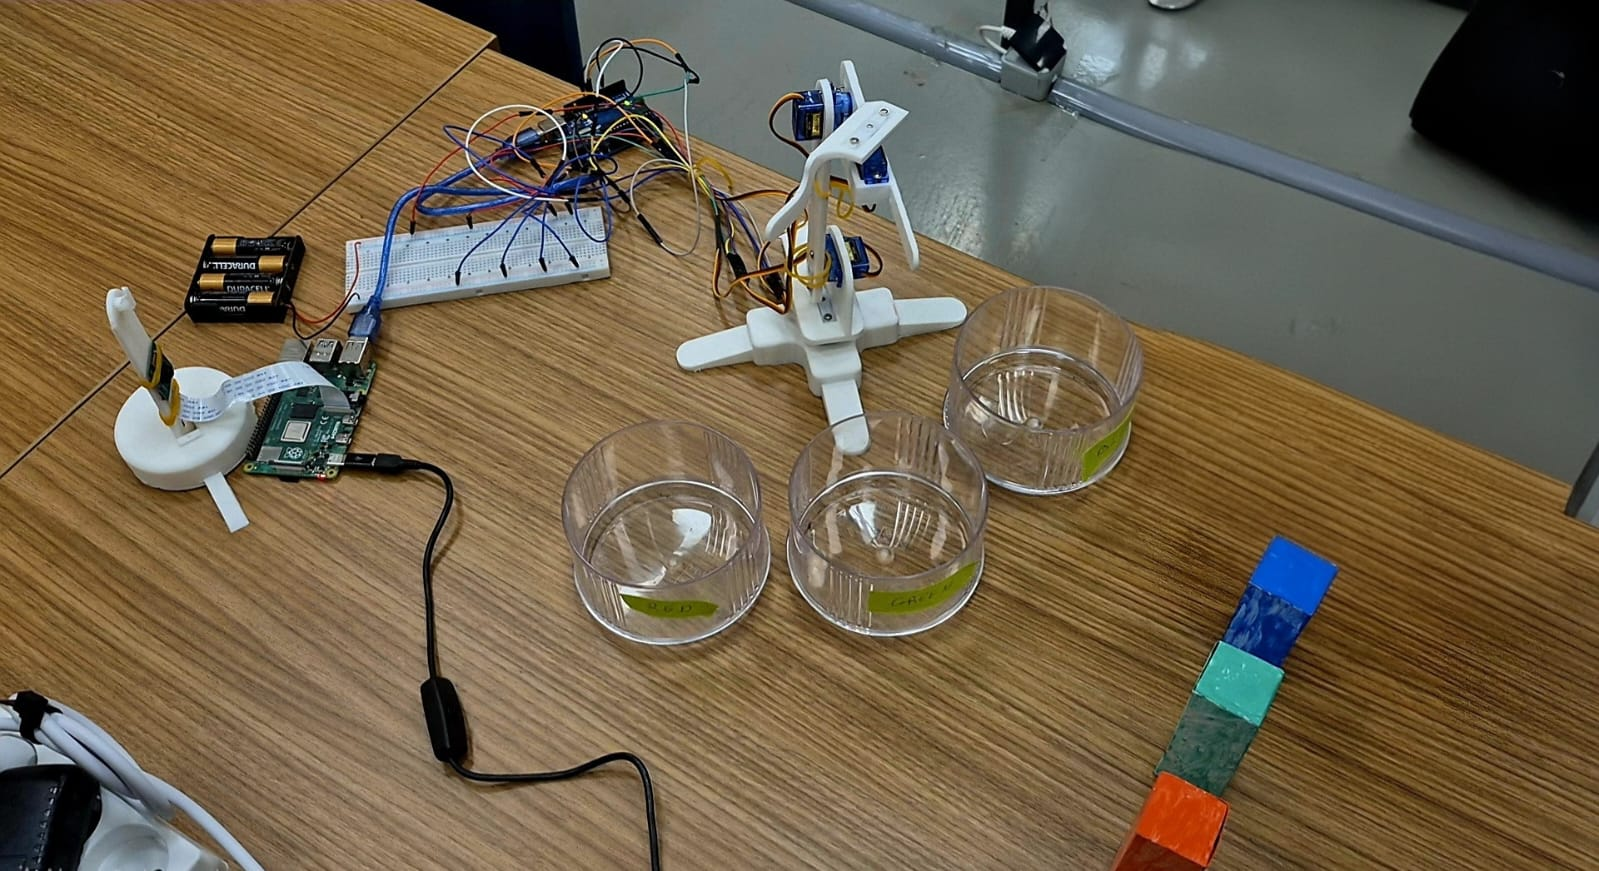
\includegraphics[width=.95\linewidth]{setup.jpeg}
\caption{Physical sorting setup. The Raspberry Pi and ribbon-connected camera are at left, with the battery holder, breadboard and Arduino behind them. The servo arm faces three collection bins. Colored test pieces are visible at lower right.}\label{fig:physical-setup}
\end{figure}


\begin{table}[htbp]\centering\small
\caption{Physical elements and documented interfaces.}
\begin{tabularx}{\textwidth}{@{}p{.31\textwidth}X@{}}\toprule
Element & Role / interface\\\midrule
3D-printed SEVEN arm & Structural assembly, base/shoulder/elbow articulation and gripper.\\
Four hobby servos & Arduino outputs: base D6, shoulder D9, elbow D10, gripper D11.\\
Arduino-compatible controller & Serial commands, inverse kinematics, joint and gripper interpolation.\\
Raspberry Pi + camera & 640$\times$480 capture, ROI segmentation and USB serial host.\\
Servo power rail & External battery supply; share signal ground with Arduino.\\
Pi supply & Separate nominal 5 V/3 A adapter as reported by the team.\\\bottomrule
\end{tabularx}\end{table}
\section{Wiring and power precautions}
The four signal wires connect to the specified Arduino digital pins. The servos must not be powered from the Arduino's logic supply in a four-servo load configuration. Servo supply ground and Arduino ground must be common for valid PWM signal references. Supply voltage under load and motor temperature were outside the scope of the model. Software limits of 0--180\,$^\circ$ are \emph{servo-command limits}, not measured structural stops.

\section{Assumptions requiring calibration}
The firmware models both shoulder-to-elbow and elbow-to-tool distances as 12 cm. Servo direction flags and trims are initially set to no reversal and zero trim. Accuracy on the physical arm depends on pivot locations, joint zero offsets, gripper travel and clearance along each route.

\chapter{Raspberry Pi Vision and Serial Communication}
\section{Camera acquisition and region of interest}
The single-frame host, \path{color_sorter_original.py}, configures Picamera2 for a 640$\times$480, \texttt{RGB888} frame, waits two seconds for camera startup and captures one image. Its rectangular region of interest (ROI) covers
\begin{equation}
(x,y)\in[220,420)\times[140,340),\qquad N_{\mathrm{ROI}}=200\cdot200=40{,}000\text{ pixels}.
\end{equation}
The script saves \texttt{classification\_result.jpg} with the ROI rectangle and \texttt{roi.jpg}. It does not use continuous tracking or locate the object's center.

\section{HSV segmentation}
The frame ROI is converted to hue, saturation and value (HSV) by OpenCV and evaluated against threshold intervals. The Python source currently invokes \texttt{cv2.COLOR\_BGR2HSV} on a frame requested in \texttt{RGB888}; if camera-channel order differs in the returned array, this convention must be verified with a known-color object. The classifier implements the bounds in Table~\ref{tab:hsv}. The two red hue windows handle the hue wraparound near the boundary between hue codes 179 and 0 in OpenCV's 8-bit HSV representation \cite{opencv}.
\begin{table}[htbp]\centering\small
\caption{Exact HSV intervals and threshold from the Raspberry Pi program.}\label{tab:hsv}
\begin{tabularx}{\textwidth}{@{}l p{.46\textwidth} X@{}}\toprule
Color & Hue range(s) & Saturation / value conditions\\\midrule
RED & 0--10 or 170--179 & $S\geq100$, $V\geq80$\\
GREEN & 35--85 & $S\geq70$, $V\geq70$\\
BLUE & 90--135 & $S\geq70$, $V\geq70$\\\bottomrule
\end{tabularx}\end{table}
For a color $c$, coverage is computed by
\begin{equation}\label{eq:coverage}
P_c=\frac{100}{N_{\mathrm{ROI}}}\sum_{u\in\mathrm{ROI}}\mathbf{1}[\mathrm{HSV}(u)\in\mathcal{H}_c], \quad c\in\{R,G,B\}.
\end{equation}
The winning class $c^*=\arg\max_c P_c$ is accepted only if $P_{c^*}\geq20\%$, equivalent to at least 8,000 matching pixels in the fixed ROI. Otherwise the result is \texttt{UNKNOWN} and no serial command is sent. This value is \textbf{mask area coverage, not a calibrated classifier confidence or a machine-learning probability}. Multiple objects or colored backgrounds can compromise this heuristic.

\section{Host-to-controller protocol}
Once a color passes the coverage threshold, the script opens \texttt{/dev/ttyACM0} at 115200 baud, waits approximately three seconds for a possible Arduino reset, and sends \texttt{CHECK COLOR}. It searches for the exact text \texttt{Route model check OK}; this tests modeled reachability, not obstacle clearance. If the check passes, the operator must answer \texttt{yes}. Only then does the script send \texttt{ARM}, wait approximately one second, and send \texttt{RUN COLOR}. The script monitors serial lines until it sees \texttt{Color route complete}, a reported error, or a 180-second timeout.

\begin{lstlisting}[language=Python,caption={Simplified control logic matching the supplied Python script.}]
color = classify_single_frame(roi)
if color not in {'RED','GREEN','BLUE'}:
    return  # no command
send('CHECK ' + color)
if 'Route model check OK' not in responses:
    return
if operator_confirms():
    send('ARM')
    send('RUN ' + color)
    monitor_until_complete_error_or_timeout()
\end{lstlisting}
\begin{note}
The original single-frame host sends RUN after a fixed delay. The capacity-aware host, \path{sort_with_slots.py}, instead waits for the ARM acknowledgement and requires the first waypoint message before it accepts route completion. A 180-second host timeout does \emph{not} transmit STOP. The controller's completion message refers to finished command interpolation, not independently sensed arrival or successful grasp.
\end{note}

\chapter{Embedded Motion Controller}
\section{Arduino structure}
The custom firmware attaches the four servos after an explicit \texttt{ARM} command. It initializes base/shoulder/elbow commands to $[105,73,60]$ degrees and the gripper to 90 degrees. It accepts manual joint commands, coordinate targets, route checks, automatic routes and manual step-through routes. The primary controls are summarized below.
\begin{table}[htbp]\centering\small
\caption{Selected commands from the team's custom Arduino protocol.}
\begin{tabularx}{\textwidth}{@{}p{.27\textwidth}X@{}}\toprule
Command & Function\\\midrule
\texttt{ARM} & Attach servos at the documented initial commanded pose.\\
\texttt{CHECK RED/GREEN/BLUE} & Validate that all route target poses pass the software IK checks.\\
\texttt{RUN RED/GREEN/BLUE} & Start an automatically advanced eight-waypoint sorting route.\\
\texttt{MANUAL COLOR} / \texttt{NEXT} & Step through the same route with explicit confirmation at each waypoint.\\
\texttt{XYZ x y z} / \texttt{M b s e} & Send Cartesian target or three explicit commanded joint angles.\\
\texttt{FK} / \texttt{POSES} / \texttt{STATUS} & Inspect computed position, target list or internal controller state.\\
\texttt{OPEN} / \texttt{CLOSE} & Operate the calibrated gripper commands.\\
\texttt{STOP} & Cancel future interpolation updates; holds the last servo outputs.\\\bottomrule
\end{tabularx}\end{table}
\section{Waypoint state sequence}\label{sec:waypoints}
\begin{table}[htbp]\centering\small
\caption{Eight-step automated sorting route (all three colors).}\label{tab:steps}
\begin{tabularx}{\textwidth}{@{}c p{.29\textwidth}X@{}}\toprule
Step & Target & Mechanical intention\\\midrule
1 & AP & Move above the pickup location with gripper open.\\
2 & PICK & Descend; command gripper to CLOSE after arrival.\\
3 & AP & Lift the object.\\
4 & HOME & Return through the home posture.\\
5 & AR / AG / AB & Move above the color-selected bin.\\
6 & DR / DG / DB & Descend into the selected drop location; command OPEN.\\
7 & AR / AG / AB & Retract above the bin.\\
8 & HOME & Return home and finish the route.\\\bottomrule
\end{tabularx}\end{table}
\section{Interpolation and timing}
Joint command values advance by at most one degree per 100 ms per positioning joint; all three are updated in each scheduled step, so the joint with the greatest required angular change determines each segment duration. Gripper commands advance by one degree per 30 ms, normally between 90 degrees (open) and 115 degrees (closed). Automatic operation introduces a one-second pause between consecutive waypoints. The program uses the Arduino \texttt{millis()} timer instead of a blocking per-degree delay. A terminal message indicates interpolation completion, not sensor-confirmed actuator movement.

\section{Safety-relevant controller behavior}
\texttt{STOP} cancels the active sequence and stops sending new interpolation commands, but it does not de-energize the servos or guarantee an emergency stop. Manual joint-angle inputs are clamped to 0--180 degrees; route IK targets are rejected outside reach and model-angle bounds. Calibration edits held in RAM are not necessarily saved across resets. These are useful software guards, but they do not replace collision detection, independent power isolation or mechanical hard-stop characterization.

\chapter{Bin Capacity Management: Three Objects per Color}\label{ch:capacity}
\section{Industrial-MVP requirement}
The host maintains an independent count for each color. For counts zero through two, it can dispatch the same firmware route to that bin. When a count reaches three, the host rejects the next request for that color before opening the serial port. The operator resets the count after emptying the bin. Each count estimates occupancy from completed routes and operator reconciliation.

\begin{table}[htbp]\centering\small
\caption{Final intended bin-capacity policy. These are the existing Arduino targets, not new calibration points.}\label{tab:bin-policy}
\begin{tabularx}{\textwidth}{@{}lccX@{}}\toprule
Color/bin & Approach pose & Drop pose & Nominal capacity and use\\\midrule
RED / Zone A & AR & DR & 3 objects; all use the same DR coordinate.\\
GREEN / Zone B & AG & DG & 3 objects; all use the same DG coordinate.\\
BLUE / Zone C & AB & DB & 3 objects; all use the same DB coordinate.\\\bottomrule
\end{tabularx}\end{table}

\section{Capacity state and invariants}
Let $\mathcal C=\{R,G,B\}$ and $n_c$ be the software-registered number of objects in bin $c$. The capacity invariant is
\begin{equation}\label{eq:counter-invariants}
 n_c\in\{0,1,2,3\},\qquad \mathrm{canSort}(c)\iff n_c<3\ \land\ \neg\mathrm{pending}.
\end{equation}
The per-color destination is independent of the counter:
\begin{equation}\label{eq:constantdrop}
  D(c,n_c)=D_c\quad\text{for }n_c=0,1,2,
\end{equation}
where $(A_c,D_c)$ denotes $(AR,DR)$, $(AG,DG)$ or $(AB,DB)$. At $n_c=3$, no command for this color is authorized. The count update is
\begin{equation}\label{eq:counterupdate}
 n_c^{+}=\begin{cases}n_c+1,&\text{on verified route completion or recovery as placed,}\\n_c,&\text{otherwise.}\end{cases}
\end{equation}
The count estimates occupancy from firmware completion. An uncertain transaction requires physical inspection before an operator resolves it.

\section{Transaction and recovery protocol}
The host controller keeps an occupancy record separate from nominal route coordinates. The controller saves a pending transaction to disk before dispatching the route. After a power or serial interruption, that record prevents an automatic retry. The next operation is blocked until an unresolved transaction is reconciled.
\begin{lstlisting}[language=Python,caption={Host-side control flow for a fixed-drop sorting transaction.},label={lst:capacity}]
def sort_color(color, state):
    if color not in {"RED", "GREEN", "BLUE"}:
        return "UNKNOWN: no action"
    if state.pending is not None:
        return "Unresolved previous operation"
    if state.count[color] >= 3:
        return f"{color} bin FULL"

    # Keep the existing Arduino pose for this color.
    # No per-slot SET or new coordinates are required.
    if not arduino_check(color) or not operator_approves():
        return "Rejected or cancelled"

    persist_pending(color)             # crash-safe intent
    if run_and_verify_completion(color):
        increment_count_and_clear_pending(color)
    else:
        preserve_pending_for_recovery()
\end{lstlisting}
Manual reset must follow actual bin emptying, not simply a desire to clear an error. On a timeout, the process must not infer that the object remained at pickup or reached the bin. An operator examines the robot and the bin, then resolves the pending transaction as \emph{placed} or \emph{not placed}. An operation lock serializes updates from competing sorter processes.

\section{Capacity-aware finite-state machine}
Figure~\ref{fig:capfsm} shows the transitions exported by the MATLAB capacity model, including the FULL guard and recovery from an interrupted transaction.
\begin{figure}[p]\centering
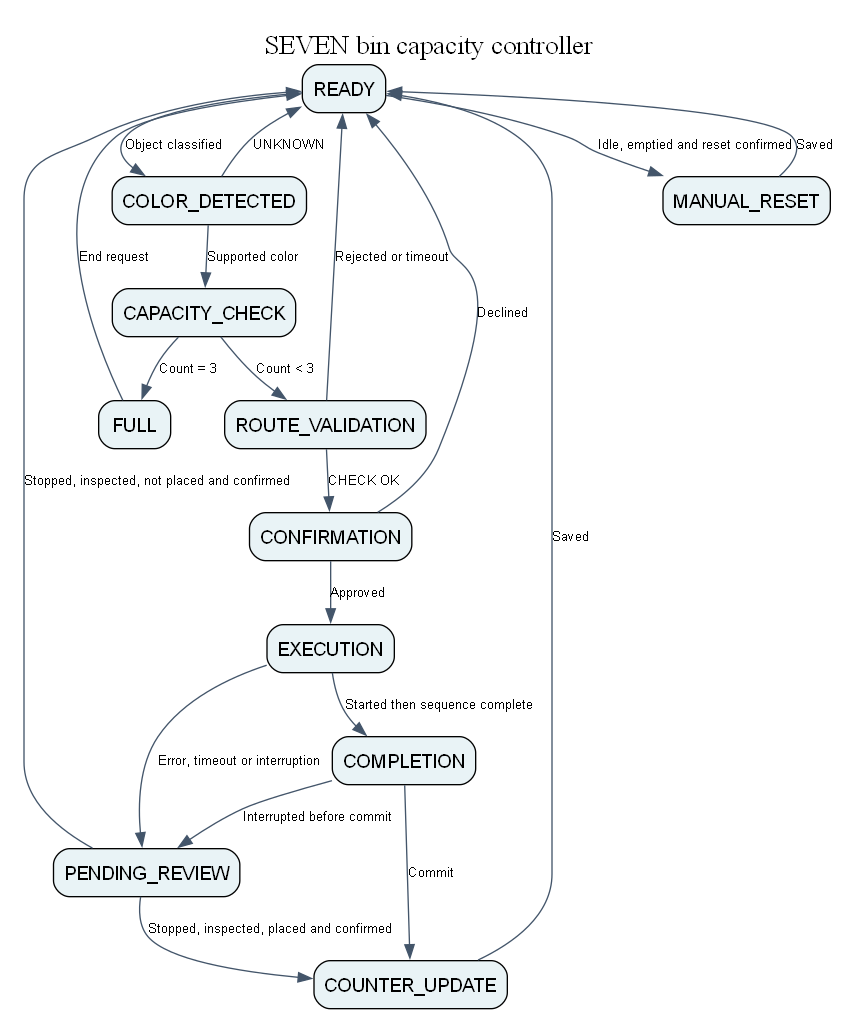
\includegraphics[width=.90\textwidth,height=.81\textheight,keepaspectratio]{docs/diagrams/slot_tracker_fsm.png}
\caption{Fixed-drop capacity model. Firmware completion commits a normal cycle. An interrupted cycle enters operator review.}\label{fig:capfsm}
\end{figure}
\FloatBarrier

\section{Controller and model evidence}
The host controller reads one destination per color from \path{config/slots.json}. The MATLAB export \path{slot_capacity_logical_example.csv} records estimated counts 1, 2 and 3 for each of the three color IDs. The exported transition table sends a count of three to FULL before serial dispatch.

All eleven host tests passed, including fourth-object rejection, independent counters, restart recovery and concurrent access. The tests use simulated serial responses.

\section{Physical feasibility of repeated same-point releases}
Each bin uses a single drop coordinate for all three releases. The clearance available for a third release depends on the object dimensions, the bin geometry and where the first two objects settle.

\chapter{Kinematic Modeling in MATLAB}
\section{Coordinate frame and nominal geometry}
The shoulder pivot is the origin of the robot coordinate system. The base angle $b$ changes the horizontal direction; shoulder angle $s$ and elbow angle $e$ determine planar reach and height. Lengths $L_1=L_2=12$ cm are nominal values copied from the custom Arduino program. MATLAB uses centimeters and degrees at the software interface and radians within trigonometric calculations.

\section{Forward kinematics}
For convenience define $\phi=s+e-\pi$, where $b,s,e$ are in radians. The horizontal reach $h$ and vertical coordinate $z$ are
\begin{align}
 h &= L_1\cos s+L_2\cos\phi,\\
 z &= L_1\sin s+L_2\sin\phi.
\end{align}
With the project's base-axis convention, the end-effector coordinate is
\begin{equation}\boxed{\mathbf p(b,s,e)=\begin{bmatrix}h\sin b\\h\cos b\\L_1\sin s+L_2\sin(s+e-\pi)\end{bmatrix}.}\label{eq:fk}\end{equation}
This expression models the nominal tool point and does not model the finger geometry, object offset, base housing or compliance.

\section{Inverse kinematics}
Given a target $\mathbf{p}=[x,y,z]^T$ from the shoulder origin, set
\begin{equation}
 r=\sqrt{x^2+y^2},\qquad d=\sqrt{r^2+z^2},\qquad b=\operatorname{atan2}(x,y).
\end{equation}
The code implements the branch
\begin{align}
 e&=\cos^{-1}\left(\frac{L_1^2+L_2^2-d^2}{2L_1L_2}\right),\label{eq:ike}\\
 s&=\operatorname{atan2}(z,r)+\cos^{-1}\left(\frac{L_1^2+d^2-L_2^2}{2L_1d}\right).\label{eq:iks}
\end{align}
These formulas correspond to the firmware's selected arm configuration; they are not a complete enumeration of all possible manipulator configurations. Validity guards additionally enforce $x\geq1$ cm, $z\geq-6$ cm, $3\leq d\leq23$ cm and commanded joint angles within $[0,180^\circ]$. The code checks the numerical reconstruction $\|\mathrm{FK}(\mathrm{IK}(\mathbf p))-\mathbf p\|<0.1$ cm.

\section{Target coordinates and model angles}
\begin{table}[htbp]\centering\scriptsize
\caption{Configured targets and corresponding modeled joint values (rounded).}\label{tab:poses}
\begin{tabular}{@{}lrrrrrr@{}}\toprule
Pose & $x$ (cm) & $y$ (cm) & $z$ (cm) & $b$ (deg) & $s$ (deg) & $e$ (deg)\\\midrule
HOME & 11.290 & -3.030 & 2.700 & 105.02 & 73.01 & 59.99\\
AP   &  3.930 & 14.680 &14.180 & 14.99 & 73.02 & 120.00\\
PICK &  3.930 & 14.680 &-4.000 & 14.99 & 34.35 & 81.80\\
AR   & 13.140 &  6.130 & 8.000 & 64.99 & 75.26 & 87.26\\
DR   & 13.140 &  6.130 & 2.000 & 64.99 & 60.27 & 75.16\\
AG   & 13.140 & -6.130 & 8.000 &115.01 & 75.26 & 87.26\\
DG   & 13.140 & -6.130 & 2.000 &115.01 & 60.27 & 75.16\\
AB   &  3.753 &-14.006 & 8.000 &165.00 & 75.26 & 87.26\\
DB   &  3.753 &-14.006 & 2.000 &165.00 & 60.27 & 75.16\\\bottomrule
\end{tabular}\end{table}
All nine positions reconstruct under numerical FK/IK to floating-point precision. The largest residual in \path{MATLAB/outputs/pose_validation.csv} is $8.93\times10^{-15}$ cm at AP. The residual tests the consistency of the forward and inverse equations before the firmware rounds the angles. The Arduino passes whole-degree values to \texttt{Servo.write}. Applying the same rounding to the nine IK solutions and recomputing FK with the nominal links gives a maximum nominal endpoint offset of about 0.12 cm across the nine targets. For PICK the offset is 0.076 cm. These calculations isolate command rounding. Backlash, load and calibration add uncertainties that the model cannot quantify.

\section{Joint-space versus Cartesian motion}
The physical controller does not independently interpolate $x,y,z$. Instead, it increments $b,s,e$ toward the IK target. Thus, even for equal start/end XY coordinates, the intermediate Cartesian path is curved. The modeled AP-to-PICK segment reaches an XY deviation of approximately 2.7313 cm from the target vertical line. A nominal endpoint reachability check is therefore insufficient to guarantee clearance along the sweep.

\begin{figure}[htbp]\centering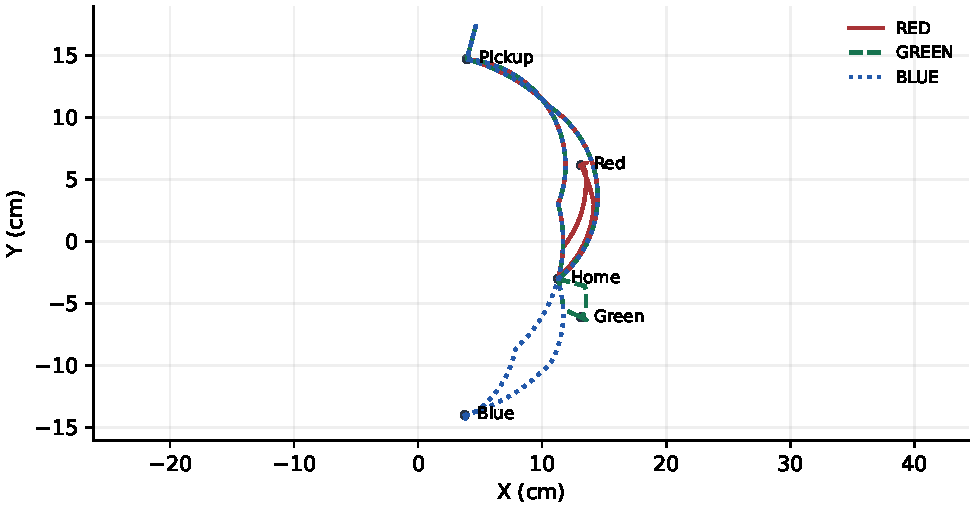
\includegraphics[width=.97\linewidth]{figures/xy_footprint.pdf}
\caption{Horizontal tool paths for RED, GREEN and BLUE. Markers identify the programmed pickup, home and drop locations. The curve at pickup shows the lateral sweep during the descent.}\label{fig:paths}\end{figure}
\begin{figure}[htbp]\centering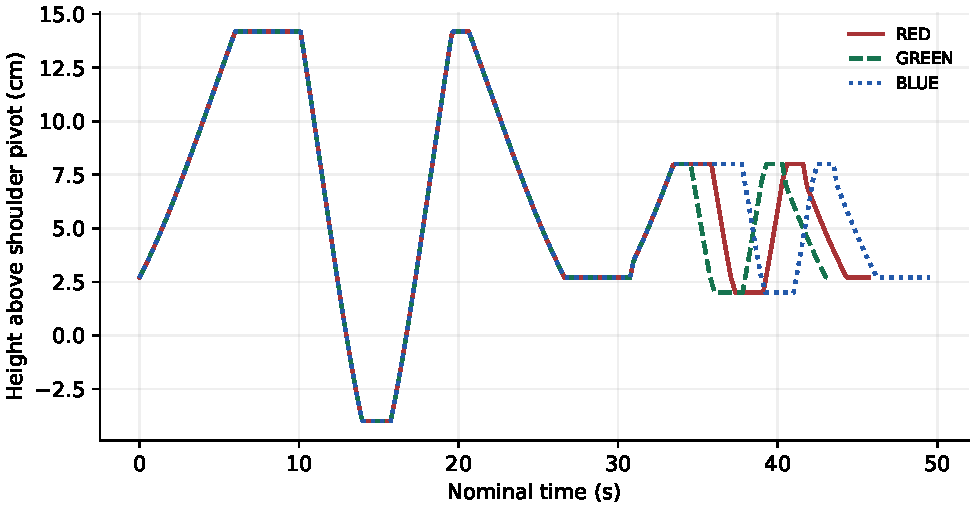
\includegraphics[width=.97\linewidth]{figures/z_over_time.pdf}
\caption{Tool height computed from the joint commands for all three routes. The pickup reaches $-4$ cm relative to the shoulder pivot and the drop reaches $2$ cm.}\label{fig:z}\end{figure}
\FloatBarrier

\chapter{Raspberry Pi and Robot Automata}
\section{States, guards and actions}
Each controller is modeled as an extended finite-state machine with a finite set of control states $Q$, an initial state $q_0$, inputs $I$, outputs $O$, and local variables $V$. A configuration $(q,v)$ records the active state and the variable values. The transition
\[
 q \xrightarrow{\ e\;[g]\;/\;a\ } q'
\]
consumes an event $e$ when guard $g$ holds. The action $a$ may emit an output, update a variable or reset a clock. An omitted guard is true. For the timed transitions, a clock valuation $\nu$ assigns a nonnegative real value to each clock. A delay of $d$ seconds advances every active clock by $d$ while the control state stays fixed. A discrete transition can reset a clock to zero.

\section{Raspberry Pi automaton}
The host starts in \texttt{START}, captures one frame in \texttt{CAPTURE} and selects the color $c$ with the greatest mask coverage in \texttt{CLASSIFY}. Coverage below 20\% leads to \texttt{NO\_COLOR}. Otherwise the host enters \texttt{CHECK\_ROUTE}, sends \texttt{CHECK} with $c$, waits 0.5 s and examines the available replies. A positive check enables \texttt{CONFIRM}. Its absence ends the attempt in \texttt{REJECTED}.

An affirmative operator response enters \texttt{ARM}, sends the arm command and resets clock $x$. When $x\geq1$ s the host enters \texttt{RUN} and sends the color route. Any other response ends in \texttt{DECLINED}. On entering \texttt{MONITOR}, the host starts a 180 s deadline. A completion line leads to \texttt{DONE}, an error line to \texttt{ERROR}, and expiry of the polling deadline to \texttt{TIMEOUT}. Each of the six exit states ends the single-frame invocation.
\begin{figure}[htbp]\centering
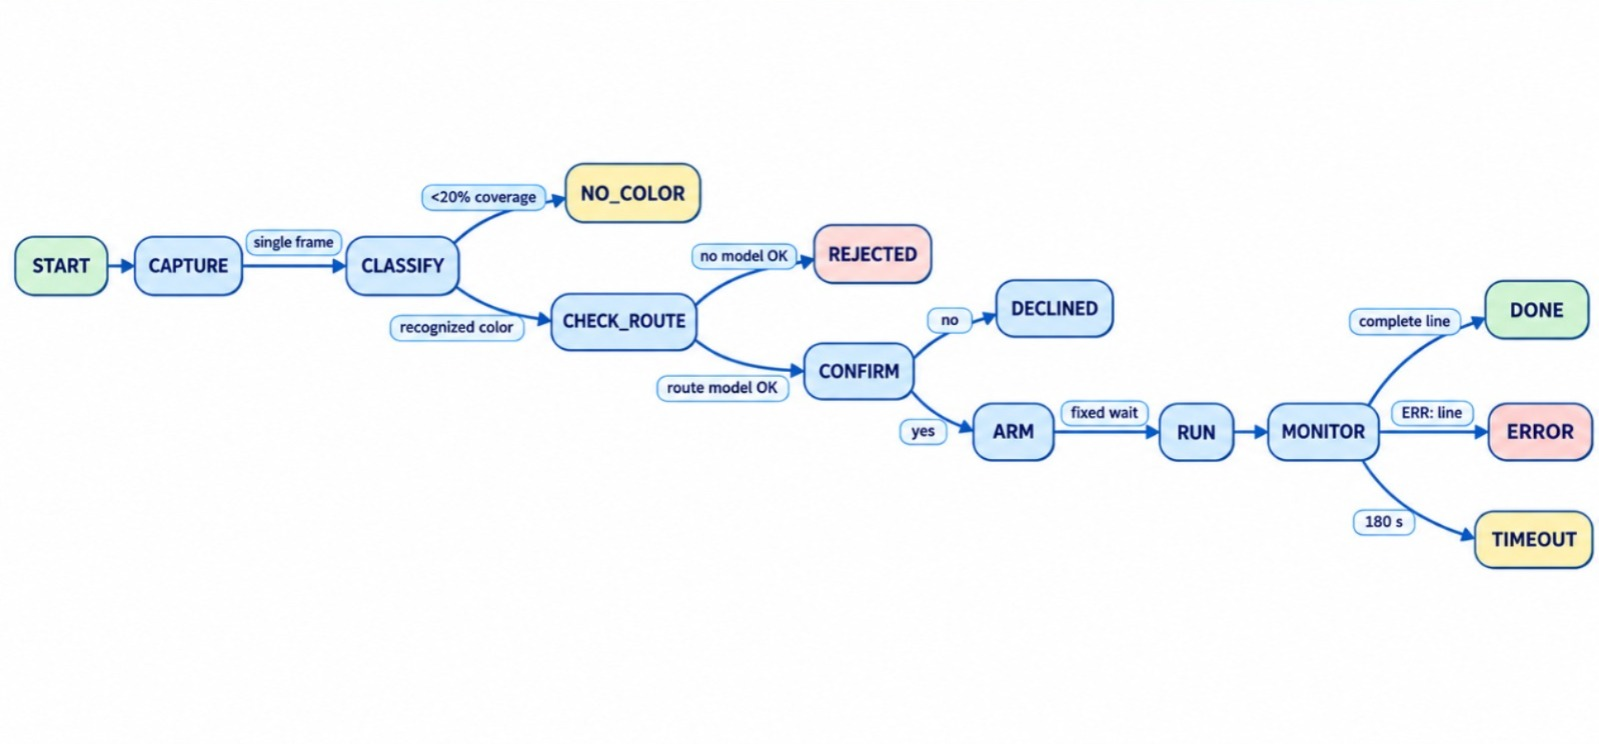
\includegraphics[width=\linewidth]{raspberri_automata.jpeg}
\caption{Raspberry Pi automaton for one sorting request. Route validation and operator approval precede the motion commands.}\label{fig:pifsm}
\end{figure}
\FloatBarrier

\section{Robot automaton}
The robot starts in \texttt{DISARMED}. Receiving \texttt{ARM} takes it to \texttt{ARMED\_IDLE}. On an accepted run, the robot sets waypoint index $k=1$. An open gripper permits an immediate transition to \texttt{MOVING}. Otherwise the robot enters \texttt{OPENING} until the opening command finishes. Arrival at PICK ($k=2$) or DROP ($k=6$) starts \texttt{GRIPPER\_ACTION}, issuing close and open commands, respectively.
\begin{figure}[htbp]\centering
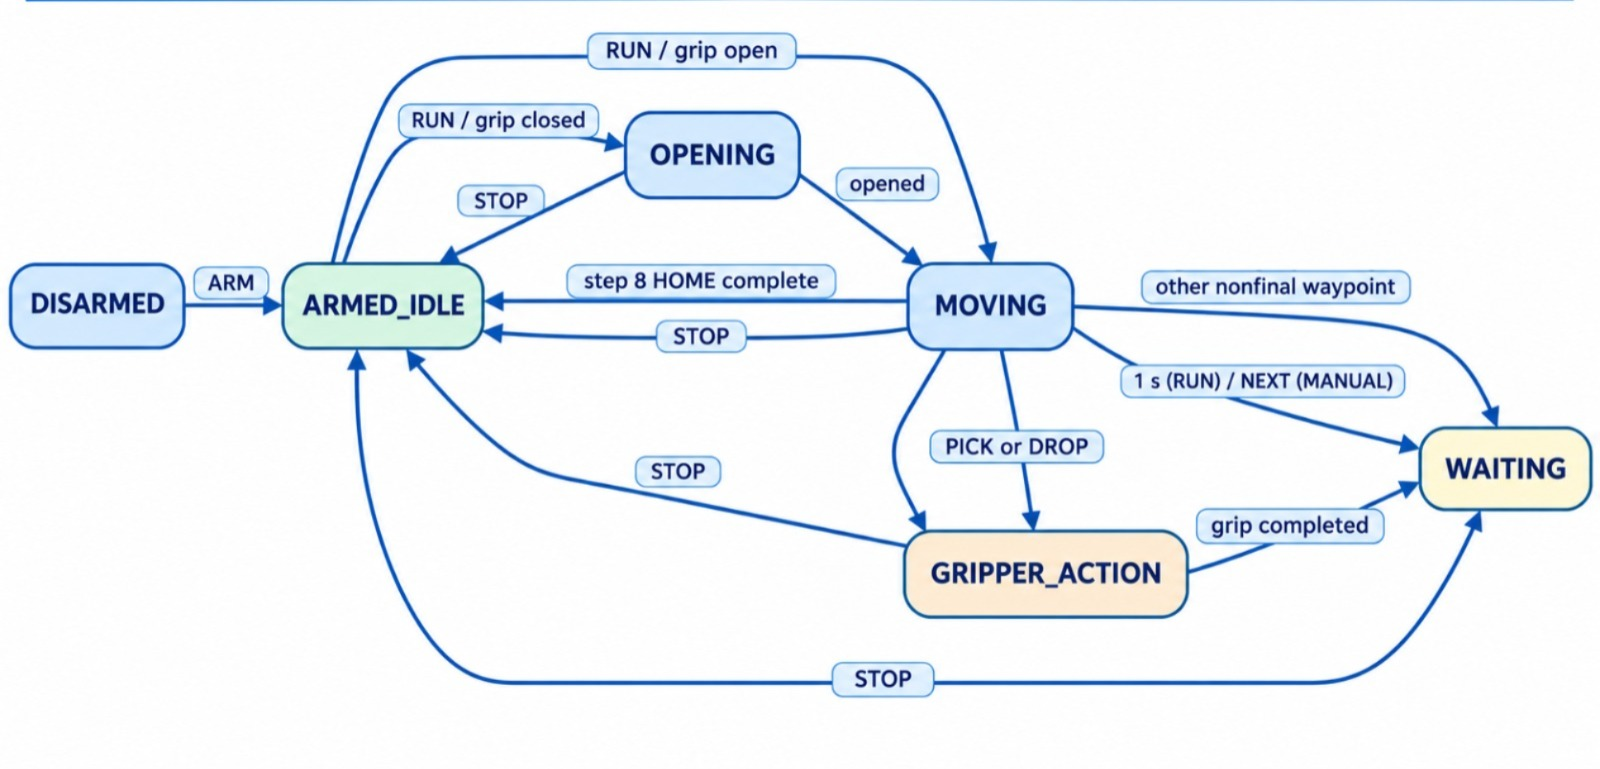
\includegraphics[width=\linewidth]{robot_automata.jpeg}
\caption{Robot automaton for joint motion, gripper actions and waypoint sequencing.}\label{fig:ardfsm}
\end{figure}

After a gripper action or an ordinary nonfinal arrival, the robot enters \texttt{WAITING} and resets clock $w$. The firmware advances as follows:
\[
 \texttt{WAITING}
 \xrightarrow{\ [(\mathrm{auto}\land w\geq1)\,\lor\,\mathrm{NEXT}]\;/\;k\gets k+1\ }
 \texttt{MOVING}.
\]
Timed auto-advance requires automatic mode. The firmware also accepts a \texttt{NEXT} command while a route is waiting, which enables manual stepping. The arrowhead labeled \emph{1 s (RUN) / NEXT (MANUAL)} in Figure~\ref{fig:ardfsm} points in the reverse direction. The transition above gives the direction in the firmware and MATLAB traces. At waypoint 8, arrival at HOME emits the completion line and returns the robot to \texttt{ARMED\_IDLE}. A \texttt{STOP} during opening, motion, gripping or waiting also returns the robot to idle and holds the existing servo outputs.
\FloatBarrier

\section{Combined automaton}
The two component diagrams describe the original single-frame host and the Arduino. The capacity-aware host adds the guards in Chapter~\ref{ch:capacity}. Figure~\ref{fig:combined-automaton} follows a sorting request from color detection to completion, rejection, error or timeout. The serial link gives an \emph{asynchronous composition}. Its control state is a pair $(q_P,q_R)$, initially $(\texttt{START},\texttt{DISARMED})$. Camera capture, operator input and waypoint timing are local events. Each changes one component while the other keeps its state. Sending a serial line places it in the channel. Its later receipt supplies an input to the peer. The nominal trace assumes ordered delivery.

For example, after the robot accepts the run, $(\texttt{MONITOR},\texttt{MOVING})$ is reachable. HOME completion changes the robot state to \texttt{ARMED\_IDLE} and emits the completion line. Reading that line moves the host to \texttt{DONE}. A host timeout changes only the host state, so the robot may still be moving.
\begin{figure}[htbp]\centering
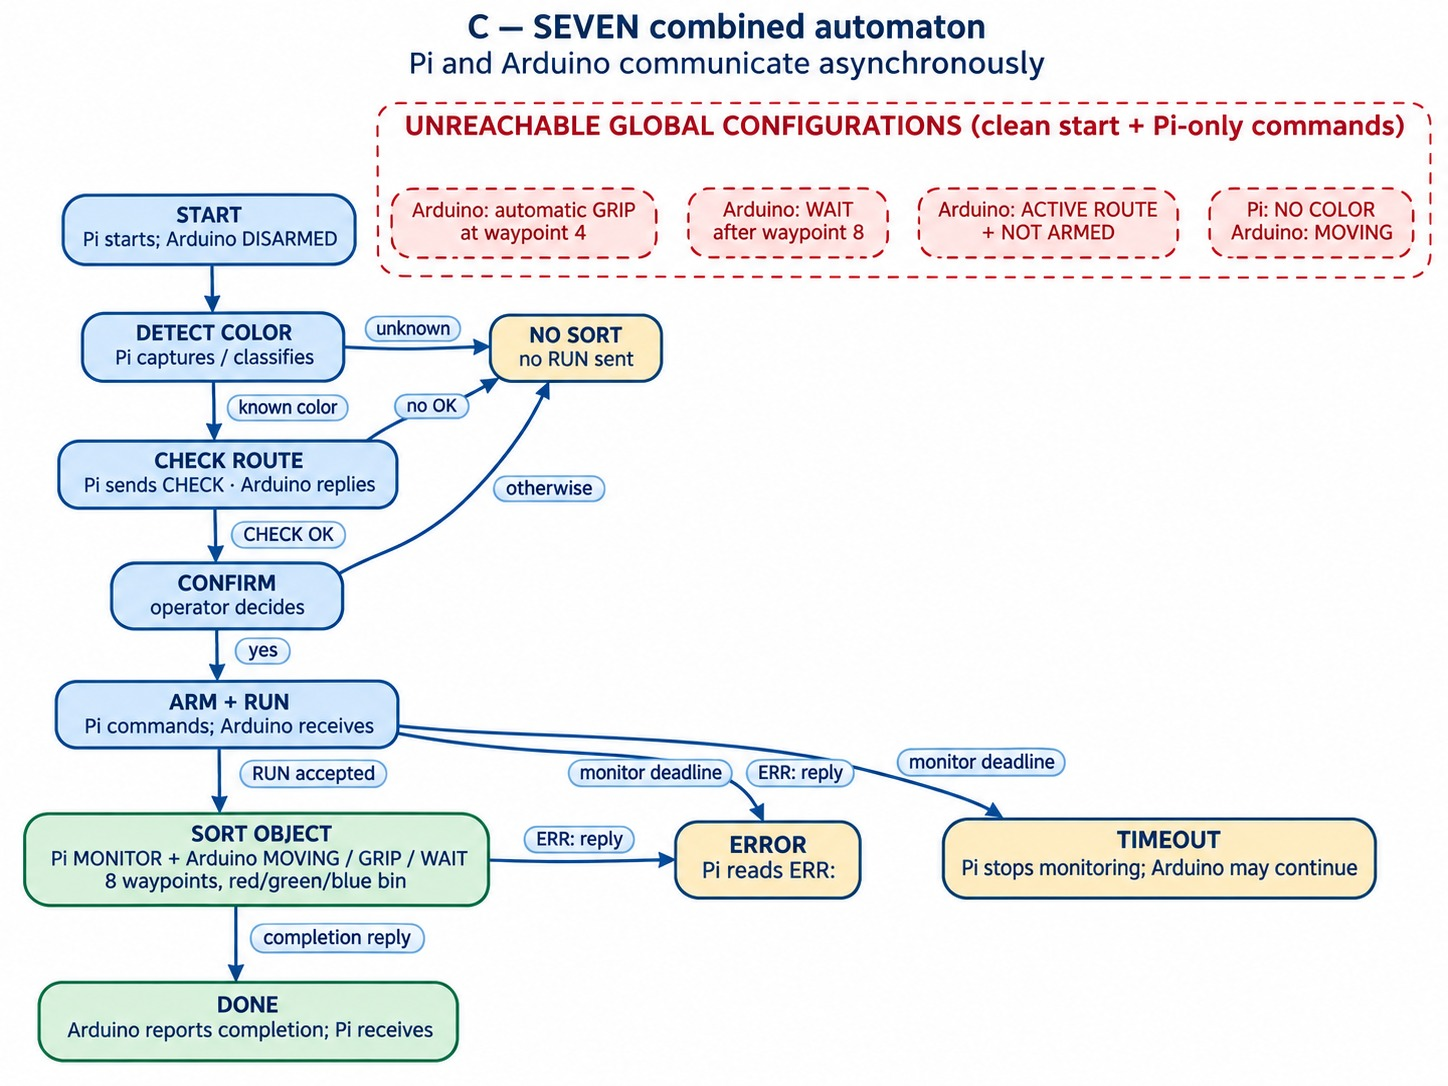
\includegraphics[width=\linewidth]{combined_automata.jpeg}
\caption{Combined Raspberry Pi and Arduino automaton. The dashed box identifies configurations that are unreachable when the robot starts disarmed and only the Pi issues commands.}\label{fig:combined-automaton}
\end{figure}
\FloatBarrier

\section{Reachability and MATLAB execution traces}
One safety property of the host is that \texttt{RUN} is unreachable on a path that exits classification through \texttt{NO\_COLOR}. The only incoming edge to \texttt{RUN} comes from \texttt{ARM}, and reaching \texttt{ARM} requires both a successful route check and approval. For each eight-waypoint automatic route, MATLAB checks that the trace contains exactly eight waypoint starts, two gripper actions (close at PICK, open at DROP), seven inter-waypoint waits and a final ARMED\_IDLE state. It also checks the final timestamp against the modeled route schedule. These assertions are checked by \texttt{seven\_fsm\_self\_test}; they are \emph{logical consistency checks} rather than hardware timing measurements.

\section{Bin-capacity state-machine integration}
The host checks capacity before dispatching the original color route. A verified firmware completion increments the estimated count and clears the pending record in one update. An interrupted run remains pending until an operator inspects the bin and resolves the transaction (Chapter~\ref{ch:capacity}).

\section{Coordination and failure handling}
The two FSMs communicate through textual serial messages; they do not share synchronized measured robot state. For instance, the Pi's host timeout warns the user but does not issue a hardware STOP command, and the Arduino's route-complete text means only that the commanded sequence finished. Robust future versions should add acknowledgement/timeout handshakes, measurable completion criteria, fault states and an independent emergency-stop mechanism.
\FloatBarrier

\chapter{Simulation and Digital Prototyping}
\section{MATLAB numerical route simulation}
The MATLAB program uses the same nominal link dimensions and target poses as the Arduino source, computes the IK targets, advances the three joint commands in steps of 1 degree every 100 ms and advances the gripper by 1 degree every 30 ms. It saves time-series CSV files containing time, three joint commands, gripper command, FK-derived $x/y/z$ and route phase. PyBullet reads these CSVs. Simulink uses the RED time and joint arrays saved in \path{seven_simulink_inputs.mat}.
\begin{figure}[htbp]\centering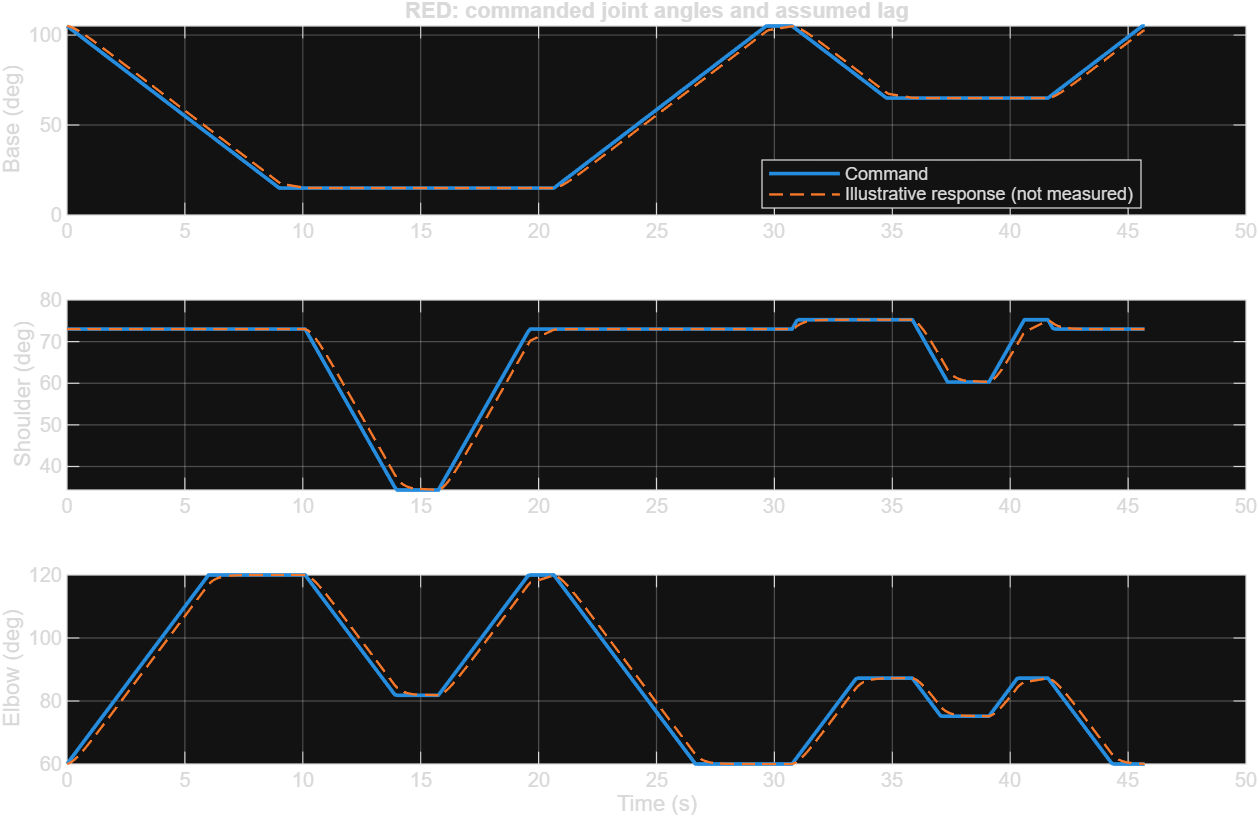
\includegraphics[width=.90\textwidth]{figures/joint_angles.png}
\caption{RED joint commands (solid) and illustrative first-order responses (dashed) for the base, shoulder and elbow.}\label{fig:redq}\end{figure}

\section{Simulink illustrative servo response}
A first-order transfer function is used to illustrate how a hypothetical servo output might follow the commanded angle:
\begin{equation}\label{eq:servo}
G(s)=\frac{\Theta_{\mathrm{assumed}}(s)}{\Theta_{\mathrm{cmd}}(s)}=\frac{1}{\tau s+1},\qquad \tau=0.35\;\mathrm{s}\quad\text{(assumed)}.
\end{equation}
The MATLAB lag calculation starts each joint at its first commanded angle. The generated Simulink transfer-function blocks use their default zero initial state, so the startup transient in the scopes also reflects that initialization. The time constant is \textbf{not identified experimentally}. The blue traces in the supplied scope captures show the response of this assumed model, while the yellow traces represent angle commands. Thus the plots support an explanatory dynamics discussion, but not claims about actual SG90 rise time, overshoot, torque or position error \cite{simulink}.
\begin{figure}[htbp]\centering
\begin{subfigure}{.49\textwidth}\centering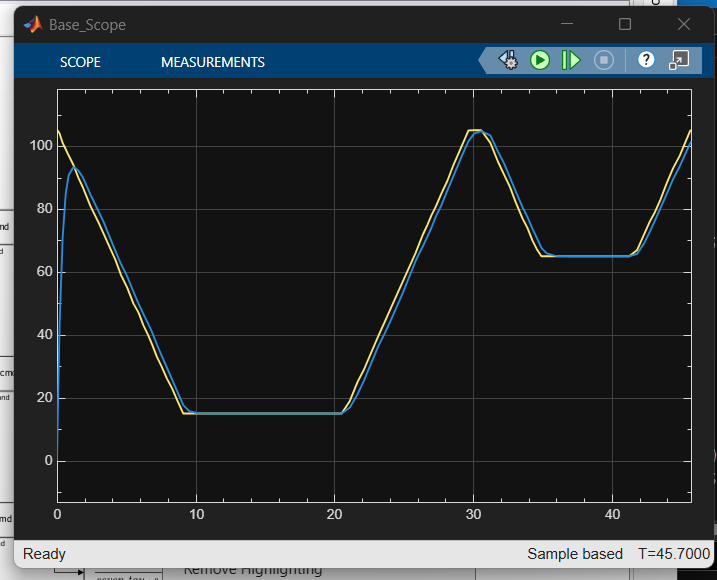
\includegraphics[width=\linewidth]{docs/evidence/Base_Scope.png}\caption{Base yaw.}\end{subfigure}\hfill
\begin{subfigure}{.49\textwidth}\centering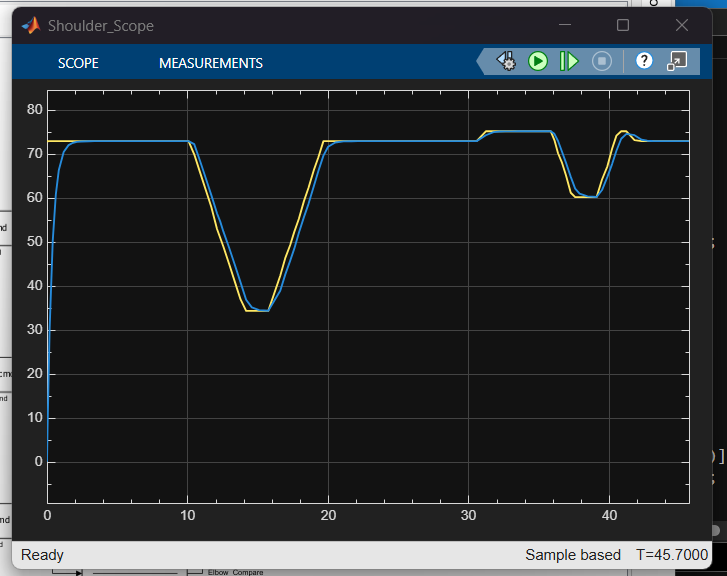
\includegraphics[width=\linewidth]{docs/evidence/Shoulder_Scope.png}\caption{Shoulder.}\end{subfigure}
\vspace{.4em}
\begin{subfigure}{.69\textwidth}\centering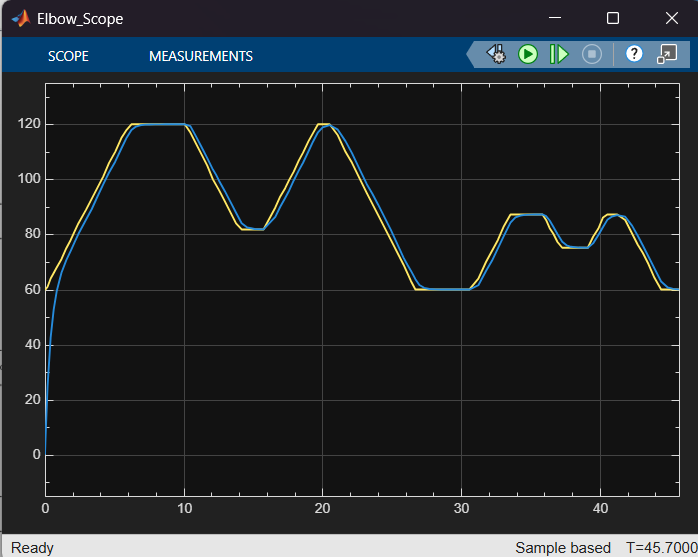
\includegraphics[width=\linewidth]{docs/evidence/Elbow_Scope.png}\caption{Elbow.}\end{subfigure}
\caption{Screenshots from the team's Simulink run: yellow commanded angle versus blue \emph{hypothetical} first-order model response.}\label{fig:scopes}\end{figure}

\section{PyBullet 3D replay and visualization}
PyBullet reads the saved command CSVs and maps the nominal joint variables into the generic URDF by
\begin{equation}
 q_{\mathrm{yaw}}=-\operatorname{deg2rad}(b),\qquad q_{\mathrm{shoulder}}=\operatorname{deg2rad}(s),\qquad q_{\mathrm{elbow}}=\operatorname{deg2rad}(e)-\pi.
\end{equation}
It repositions the visual jaws and uses a scripted object attachment at pickup followed by scripted release at the destination. The 3D geometry is a generic articulated proxy, not a reconstructed STL assembly. Position consistency is tested against the same analytical FK; rigid-body dynamics and contact-based grasp success are \emph{not} validated by these scripted motions \cite{pybullet}.
\begin{figure}[htbp]\centering
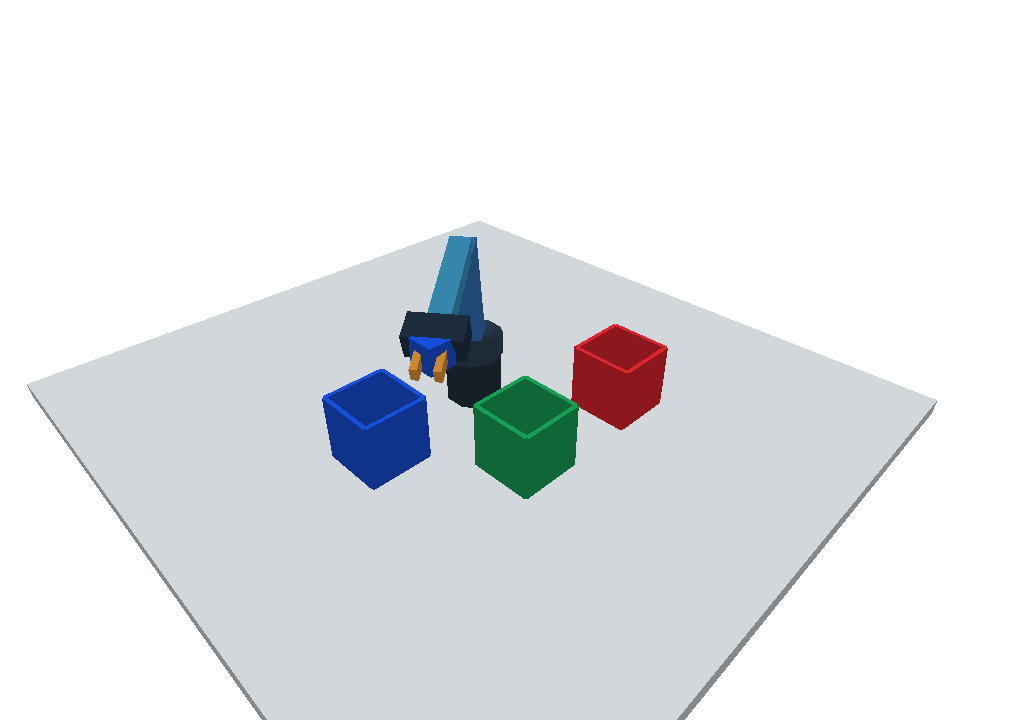
\includegraphics[width=.80\textwidth]{figures/SEVEN_PyBullet_BLUE.png}
\caption{BLUE route during scripted transfer in the PyBullet GUI replay of the MATLAB commands.}\label{fig:pybullet}\end{figure}
\section{Why each simulator was used}
MATLAB establishes consistency of geometric calculations, the finite-state-machine generator documents control behavior, Simulink illustrates an assumed actuator time response, and PyBullet shows the command sequence spatially. No MATLAB 3D animator, Simscape import or STL model is required in the final submission package. The toolchain is therefore intentionally simple and reproducible.

\chapter{Verification, Testing and Results}
\section{Verification strategy}
The setup photograph documents the installed hardware for FR-01. Section~\ref{sec:vision-check} tests the classification decision in FR-02. The host tests exercise route checking and approval (FR-03 and FR-04) and bin capacity and destination selection (FR-09 and FR-10). The route traces, pose calculations and replay cover the sequence, gripper commands and models in FR-05 through FR-08.
\begin{table}[htbp]\centering\small
\caption{Evidence-based validation matrix.}\label{tab:validation}
\begin{tabularx}{\textwidth}{@{}p{.24\textwidth}p{.38\textwidth}X@{}}\toprule
Test & Outcome/evidence & Interpretation\\\midrule
Camera decision & All seven synthetic frames produced the expected class (Section~\ref{sec:vision-check}). & Tests the HSV masks, crop and threshold.\\
MATLAB nine-pose IK/FK & Reconstructed targets at floating-point roundoff. & Equations and target table internally consistent.\\
MATLAB route exports & Three command files end at HOME at the times in Table~\ref{tab:results}. & Nominal route schedule.\\
MATLAB FSM traces & Each contains eight moves, two gripper actions and seven waits, ending in ARMED\_IDLE. & Model event sequence.\\
PyBullet GUI and headless & All three routes triggered grasp and release in both modes. & Agreement of replay events across modes.\\
Simulink scopes & Three command/response captures. & Illustrative first-order joint tracking.\\
Host capacity tests & All eleven tests passed. & Fixed destinations, capacity guards and state recovery.\\\bottomrule
\end{tabularx}\end{table}

All three MATLAB self-tests passed on a separate copy of the submitted model. The checks covered pose reconstruction, gripper sequencing, route timing, the two controller state machines and the capacity transitions for completion, recovery and reset.

\section{Vision decision at the acceptance threshold}\label{sec:vision-check}
Seven synthetic frames exercised the production \texttt{detect\_color} routine with a simulated camera. Each frame was $640\times480$ pixels with a black background. Colored patches were specified in HSV with $S=V=255$, converted to BGR and supplied at the camera-array boundary. The normal crop, thresholding and winner selection then ran in OpenCV. Table~\ref{tab:vision-check} gives the observed outputs.

\begin{table}[htbp]\centering\small
\caption{Classification results for controlled input frames. Coverage is the largest color-mask percentage inside the ROI.}\label{tab:vision-check}
\begin{tabularx}{\linewidth}{@{}X r l@{}}\toprule
Input & Coverage & Output\\\midrule
8,000 red pixels inside, hue 5 & 20.0000\% & RED\\
8,000 red pixels inside, hue 175 & 20.0000\% & RED\\
8,000 green pixels inside, hue 60 & 20.0000\% & GREEN\\
8,000 blue pixels inside, hue 120 & 20.0000\% & BLUE\\
7,999 green pixels inside, hue 60 & 19.9975\% & UNKNOWN\\
8,000 blue pixels outside, hue 120 & 0\% & UNKNOWN\\
Black frame & 0\% & UNKNOWN\\\bottomrule
\end{tabularx}
\end{table}
A single pixel changes the decision at the configured boundary. The outside-ROI case confirms that a large colored patch elsewhere in the frame cannot trigger sorting. Camera exposure, reflections and object appearance remain sources of uncertainty on the bench.

\section{Numerical route results}
\begin{table}[htbp]\centering\small
\caption{Reproduced MATLAB and PyBullet command-model results (not observed hardware times).}\label{tab:results}
\begin{tabular}{@{}lrrrrr@{}}\toprule
Color & Samples & Duration (s) & Grasp (s) & Release (s) & XY drift (cm)\\\midrule
RED & 430 & 45.7 & 14.8 & 38.1 & 2.7313\\
GREEN & 404 & 43.1 & 14.8 & 36.8 & 2.7313\\
BLUE & 468 & 49.5 & 14.8 & 40.0 & 2.7313\\\bottomrule
\end{tabular}\end{table}
The MATLAB FSM starts closing at 14.00 s on every route. Closing takes 0.75 s, so the replay attaches the object at 14.75 s (14.8 s at the displayed precision). Table~\ref{tab:results} gives the scripted attachment and release times. The GREEN route finishes 6.4 s before BLUE. The waypoint logs locate this difference in two moves. BLUE takes 3.2 s longer to reach the bin approach from HOME and another 3.2 s longer on the return. Its base turns about $60^\circ$ from HOME to the approach, compared with $10^\circ$ for GREEN. Both routes have the same grip actions and seven one-second pauses. These route times start at motion dispatch and exclude camera startup, classification and operator approval.

Across the three routes, \path{MATLAB/outputs/route_summary.csv} gives a maximum horizontal deviation of 2.731 cm during pickup descent and 0.200 cm during drop descent. The largest tool-position difference between the commanded and assumed lagged trajectories is 1.662 cm on every route with $\tau=0.35$ s. The GUI and headless PyBullet runs each report a maximum tool-frame discrepancy of $9.9\times10^{-7}$ cm for each color relative to analytical FK. This measures agreement between software coordinate models.

\section{Interpretation and main engineering finding}
The MATLAB export and the independent PyBullet transform calculation agree on the nominal tool coordinates. The modeled pickup descent, however, moves horizontally by approximately 2.73 cm despite sharing start/end XY coordinates. The surrounding workspace must therefore accommodate a curved approach even when the programmed descent begins and ends at the same horizontal position.

\chapter{Discussion and Future Work}
\section{Strengths}
The working MVP integrates a complete sense--decide--act pipeline, explicit human confirmation, a route guard, nonblocking Arduino motion, interpretable mathematical modeling, FSM-based documentation and multiple independent software consistency checks. Independent bin counters allow the host to reject a fourth request for one color while continuing to accept requests for the others. The code also preserves a clear separation between the team's custom firmware and the open-source hardware design.
\section{Known limitations}
\begin{itemize}
\item \textbf{Single-frame HSV rules:} performance may vary with lighting, exposure, shading and backgrounds. The ROI coverage threshold is heuristic.
\item \textbf{Joint-space sweeps:} valid endpoints do not imply collision-free paths; the predicted pickup lateral drift is especially relevant.
\item \textbf{No force/position sensing at the gripper:} an interpolated gripper command does not prove an object is held.

\end{itemize}

\section{Conveyor-fed sorting by material}
An industrial MVP would receive items as they arrive on a conveyor belt. The belt could index one item at a time to the arm's existing pickup point. A presence sensor wired to the Arduino would detect each arrival. The Arduino would stop the belt through a motor driver and signal the Raspberry Pi to classify the item. Once the arm finishes the route and returns to HOME, the controller could admit the next item. This lets the system respond to arrivals in real time while keeping the object stationary during pickup. The modeled arm cycles take 43.1--49.5 s, so the feed rate would need to follow the measured cycle time or allow items to queue upstream.

Material sorting would require a separate identification step at the pickup station. For a feed restricted to known steel and plastic parts, an inductive sensor could flag metal while the presence sensor confirms that an item is in position. With a mixed feed, a metal signal alone cannot identify steel, and a nonmetal reading cannot establish that an item is plastic. The controller would therefore need a validated test for each accepted material and a route for unidentified items. The Raspberry Pi could then select the destination by material and retain color as a secondary criterion where useful.

\chapter{Conclusion}
SEVEN demonstrates the core sense--decide--act functions of an industrial color-sorting application through a working educational robotic-arm MVP. The Raspberry Pi classifies color inside a fixed region, the Arduino performs a color-dependent eight-waypoint pick-and-place sequence, and the modeling chain independently documents the intended motions. The nine configured target poses pass numerical forward/inverse-kinematics reconstruction; MATLAB-command durations are 45.7, 43.1 and 49.5 seconds, while Simulink illustrates assumed servo dynamics and PyBullet replays the route spatially. The modeled 2.73 cm lateral drift during pickup descent shows why clearance depends on the full path.

The host controller maintains independent three-object counts at the existing drop coordinates. The MATLAB capacity model records the expected count progression, and eleven host tests verify the software behavior.

\begin{thebibliography}{9}
\bibitem{seven} T. Sel\c{c}uk Y\"uksel, \emph{Seven --- 3-DOF Arduino Robotic Arm}, public project repository and assembly guide, GitHub. \url{https://github.com/elevenMiles/Robotic_Arm_Seven}. Accessed November 2026. Hardware design attribution; the team's custom firmware differs from the upstream commands.
\bibitem{opencv} OpenCV, \emph{Thresholding Operations using inRange}, OpenCV documentation. \url{https://docs.opencv.org/4.x/da/d97/tutorial_threshold_inRange.html}. Accessed November 2026.
\bibitem{simulink} MathWorks, \emph{Transfer Fcn block}, Simulink documentation. \url{https://www.mathworks.com/help/simulink/slref/transferfcn.html}. Accessed November 2026.
\bibitem{pybullet} E. Coumans and Y. Bai, \emph{PyBullet Quickstart Guide}, Bullet Physics project documentation. \url{https://github.com/bulletphysics/bullet3/blob/master/docs/pybullet_quickstart_guide/PyBulletQuickstartGuide.md.html}. Accessed November 2026.
\bibitem{source} SEVEN team, \emph{Original Arduino and Pi source, optional capacity-controller archive, MATLAB and PyBullet outputs, and associated test records}, project submission materials inspected November 2026.
\end{thebibliography}

\appendix
\chapter{Reproducibility and Project Navigation}
\section{Delivered source-code components}
The engineering package separates the embedded controllers from the offline models \cite{source}.
\begin{lstlisting}[caption={Relevant source layout (excerpt).}]
SEVEN_Color_Sorting_Submission/
  Original_Source_Code/
    Arduino/SEVEN_color_sorter_original/*.ino
    RaspberryPi/color_sorter_original.py
    RaspberryPi/sort_with_slots.py   # fixed-drop controller

  config/slots.json            # one destination per color
  MATLAB/
    run_SEVEN_project.m
    seven_self_test.m
    seven_fsm.m
    seven_fsm_self_test.m
    seven_slot_fsm.m           # fixed-drop capacity model
    seven_slot_fsm_self_test.m
    seven_build_simulink.m
    src/ ...
    outputs/{RED,GREEN,BLUE}/commands.csv
  PyBullet/
    simulate.py
    test_urdf.py
    robot/seven_kinematic.urdf
    trajectories/{RED,GREEN,BLUE}_commands.csv
  docs/
    FINITE_STATE_MACHINES.md


\end{lstlisting}
\section{Windows/Python verification}
The following commands use the project root as the initial working directory.
\begin{lstlisting}[language=bash]
py tools/preflight.py
py -m unittest discover -s tests -v
py PyBullet/simulate.py --verify-only --all
cd PyBullet
py -m pip install -r requirements.txt
py test_urdf.py
py simulate.py --color RED
py simulate.py --color GREEN
py simulate.py --color BLUE
\end{lstlisting}
\section{MATLAB and Simulink verification}
The MATLAB verification sequence uses \texttt{MATLAB} as its working directory.
\begin{lstlisting}
run_SEVEN_project
seven_self_test
seven_fsm
seven_fsm_self_test
seven_slot_fsm
seven_slot_fsm_self_test
seven_build_simulink
\end{lstlisting}
The MATLAB run writes pose checks, route summaries and per-color plots under \path{MATLAB/outputs}. The \path{fsm} subdirectory contains the timed route traces and capacity transitions. PyBullet reads the exported commands for the 3D replay.
\section{Reproducibility boundaries}
The package check verifies source hashes, the generic robot model and byte-identical trajectory copies for all three colors. PyBullet uses the MATLAB exports when available and otherwise reads \path{PyBullet/trajectories}. The host tests use synthetic inputs and simulated serial responses. The MATLAB run predicts motion from joint commands.
\end{document}
